\newpage
\section{Decoding}
Discrete gate integrated chips are used throughout the board for decoding and demultiplexing address, data and control lines.

    \subsection{Programmable Logic Device - PAL16L8}
    Programmable Array Logic (PAL) is a type of Programmable Logic Device (PLD) used to implement logical functions. \cite{pal} PALs comprise of an AND gate array followed by an OR gate array, as shown in Figure \ref{fig:pal}.\n
    16L8s were programmed to be used throughout the board to implement the various functionalities required in the system.

        \begin{figure}[h]
            \begin{center}
                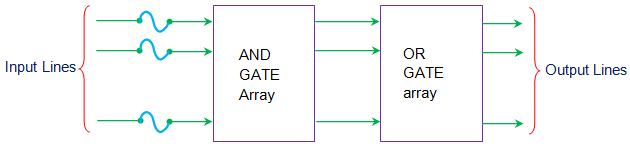
\includegraphics[width=0.9\textwidth]{figures/pal.png}
                \caption{8086 Microprocessor} \label{fig:pal}
            \end{center}
        \end{figure}


    \subsection{Programming the PLD}
    VHSIC Hardware Description Language (VHDL) was used to program the different logical functions. The modules used for the nine (9) 16L8s used in the system are implemented in Appendix \ref{appendix:code}.

    \subsection{Pinouts}
    Refer to Appendix \ref{appendix:pinouts} for the pinouts of the chip.
